\chapter{User study} \label{chapter:user_study}

    To guide future efforts, we decided to perform a user study to directly gauge the users' views. Overall, our study had three main goals:
    
    \begin{itemize}
        \item confirming the importance of campus navigation for certain user groups (first year students, aspiring high school students and parents, other one-time campus events participants)
        
        \item understanding the students' campus navigation needs: what they're currently using, and what they are missing
    
        \item getting feedback regarding our four prototypes, described in the previous chapter
    \end{itemize}

\section{Past studies}

    As stated previously, we have based our implementation decisions upon known and established state of the art solutions, as well as previous related studies.
    
    \subsection{ACS UPB Mobile}
    
        One notable study has been performed by us for the previous paper, "Design and Implementation of a Cross-Platform Mobile Application That Facilitates Student Collaboration"\cite{alexandru2020acsupbmobile}. There are a few key points that we've used from this existing user study from 2019, which had over 200 answers.
        
        Firstly, we know that, although the majority (roughly 80\%) of students in our target user group use an Android phone, the iOS demographic is still significant enough to warrant investing effort in a cross-platform solution.
        
        Secondly, over 35\% of student responders prefer to use English as the main language of their mobile OS. This, paired with the fact that the faculty welcomes foreign students, is again significant enough to justify the need for a localized app that supports at least two languages: English and Romanian. Inclusiveness is a top priority, therefore students of all backgrounds should have access to our campus navigation tool.
        
        Finally, we also have to note that, based on this prior study, a map function was second to last on a usefulness scale for student responders. As highlighted previously in section \ref{1:functionalities}, we agree that the usefulness of a tool that simply provides navigation instructions will decrease significantly over time, as a student learns the locations of their classes. As such, in the same chapter we propose additional functionalities that would keep the tool relevant even as time passes.
    
    \subsection{UPB Campus}
    
        A similar study was also done for the UPB Campus app, also in 2019, by Diana Scurtu\cite{scurtu2020upb}. From there, we learn that, out of over 100 surveyed students (a majority of which were first year students), a whooping 68\% consider it difficult to find some locations in the campus. In terms of methods used by students to go around campus, 44\% prefer to ask for directions, while the rest are equally split (28\% each) between using the campus map and using a GPS mobile app. Finally, roughly 88\% of survey responders believed that an application for the university campus would be useful.

\section{Methods}

    For our study, we chose to use a mix of research approaches. The base of our research consisted of \textbf{analysing previous studies}, as well as using \textbf{observation} directly throughout six years studying at \acrshort{acs} and interacting with the students and the campus. Furthermore, we sent out a \textbf{survey} that received over 100 responses, and conducted 1:1 \textbf{interviews} with university students, professors and even high school students who aim to apply at \acrshort{upb}.
    
    Thanks to the mostly-online medium we've found ourselves in the past couple of years due to the pandemic, most of our communication was done over the internet. The survey consisted of a \textit{Google Form}\footnote{\url{http://forms.google.com/}} that was shared via \textit{WhatsApp}\footnote{\url{https://www.whatsapp.com/}} to various students' groups. Most interviews were conducted over a \textit{Microsoft Teams}\footnote{\url{https://teams.microsoft.com/}} video call, with some taking place face-to-face or over a chat app (\textit{WhatsApp}, \textit{Facebook Messenger}\footnote{\url{https://messenger.com/}}, \textit{Telegram}\footnote{\url{https://telegram.org/}}).
    
    The data from the survey was extracted into a \textit{Microsoft Excel}\footnote{\url{https://www.microsoft.com/en-us/microsoft-365/excel}} spreadsheet, normalised and used to generate charts and other correlational statistics (see section \ref{4:results} below).


\section{Results} \label{4:results}

    \subsection{Survey}

        Our survey included a variety of different questions, while still being short enough to not discourage students from filling it out. As such, we have received over 100 responses in the span of one week. We have used open-ended, as well as multiple choice questions (both with only one as well as with multiple possible responses) and a Likert scale.
        
        Firstly, in order to gauge how common of an issue finding a campus location is, differently from previous questionnaires, we have asked students what are the reasons they have been late for a class. Figure \ref{4:fig:late_to_class} shows the number of students (out of 103 responses) who chose each answer in a multiple-choice, checkbox-style question allowing multiple answers. There, we can see that not finding the classroom is the second most common reason identified by the students with a 54\% agreements, after waking up late (63\%). Other reasons included the class before going overtime and being stuck in traffic, which 44\% and 33\% of students relating to, respectively.
        These results work to confirm our assumption that not being able to efficiently navigate through campus may affect the students' ability to get from one class to the other in time.
            
        \begin{figure}[!ht]
            \centering
            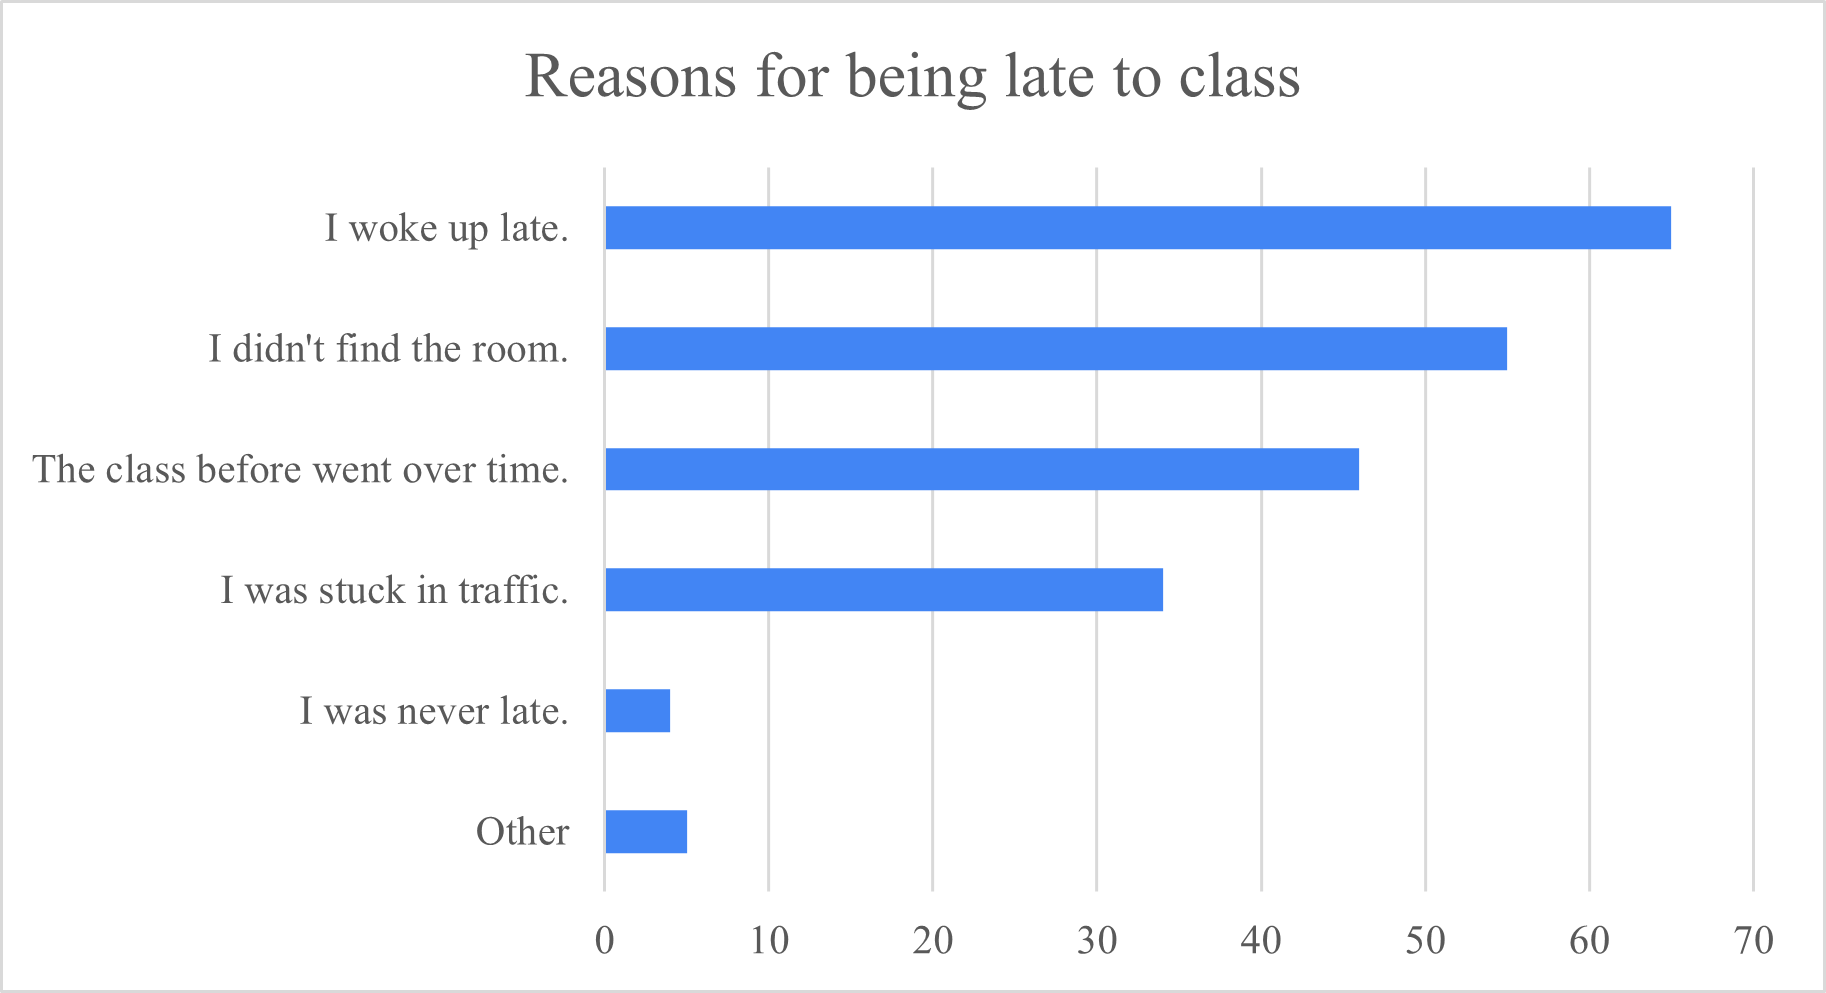
\includegraphics[width=\textwidth]{figures/charts/late_to_class.png}
            \caption{Students' reasons for being late to class}
            \label{4:fig:late_to_class}
        \end{figure}
        
        \newpage
        
        Next, we asked students what tool or approach they are using when they need to navigate through campus. The results here closely matched the one from the study made in 2019 for UPB Campus\cite{scurtu2020upb}. Figure \ref{4:fig:navigation_methods} shows the result of another checkbox-style question, with the x-axis representing the number of students who checked a specific answer. Notably, many students (roughly 40\%) prefer to use a mix of multiple methods rather than just one. The majority of student responders (49\%) prefer to ask colleagues or someone else for directions. Some students use a photo of the map or the freshman's guide\footnote{\url{https://www.slideshare.net/vladposea/ghidul-bobocului-de-la-facultatea-de-automatica-si-calculatoare-vers-20112012}} (44\%), while others make use of well-established navigation apps such as Google Maps (44\%) and Apple Maps (3\%). Finally, although it has been more than two years since the launch of the UPB Campus app, only 2 students mentioned using it for campus navigation.
            
        \begin{figure}[!ht]
            \centering
            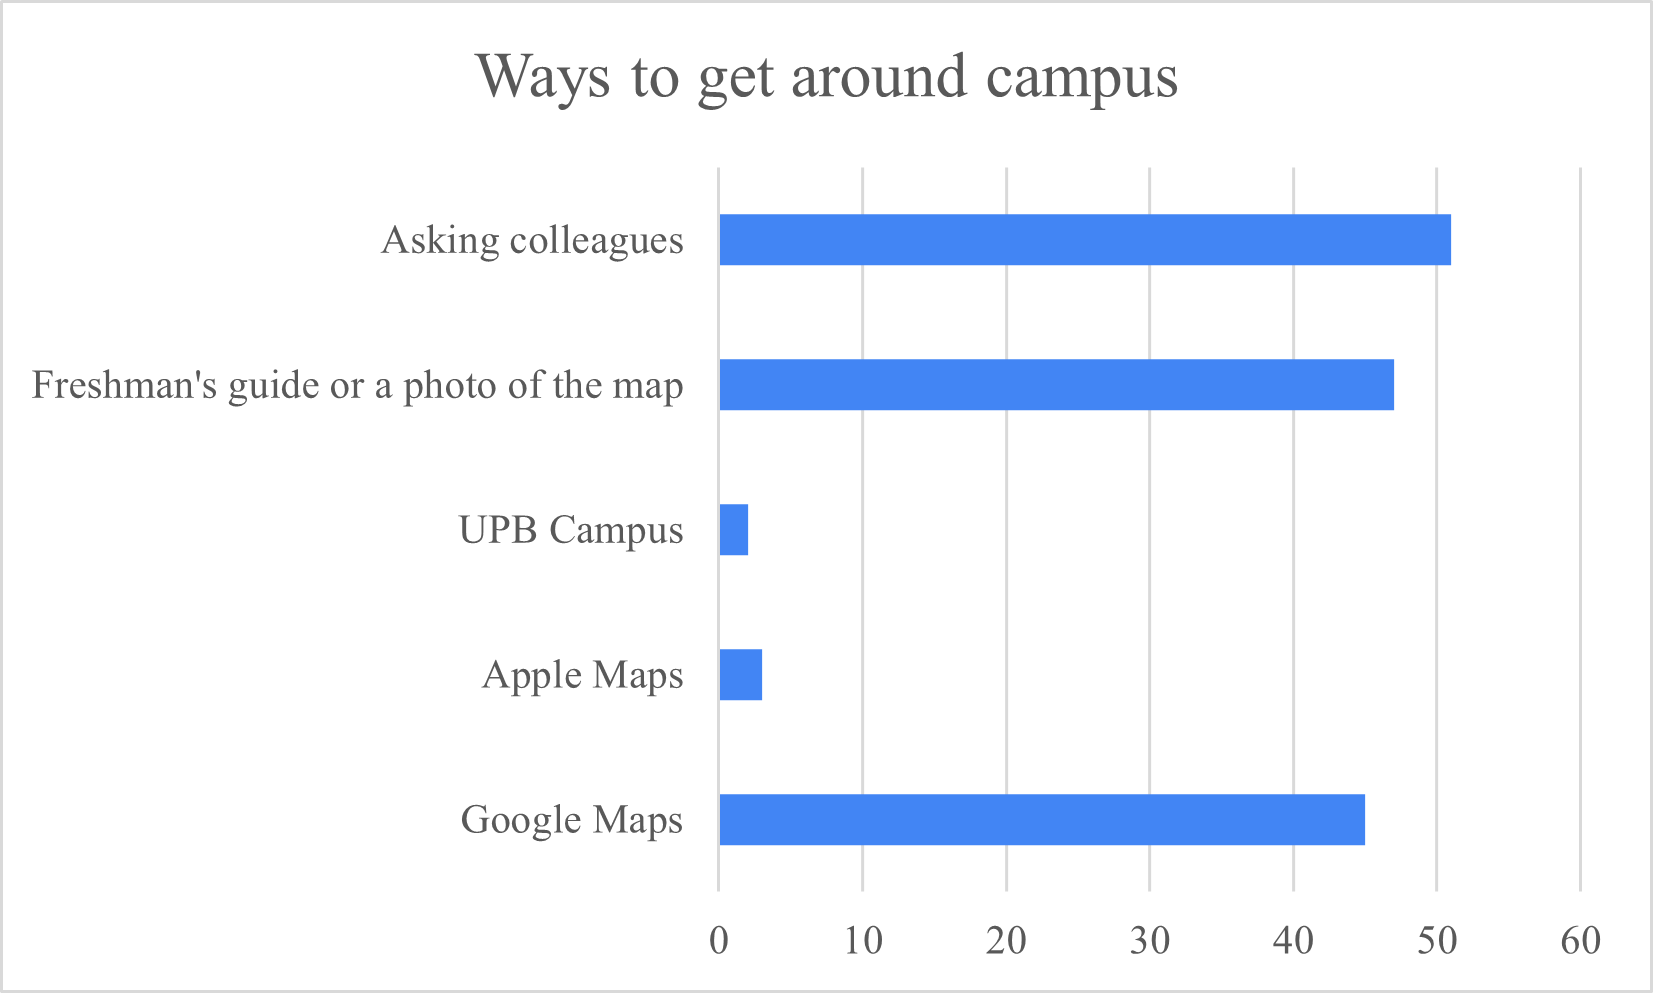
\includegraphics[width=\textwidth]{figures/charts/navigation_methods.png}
            \caption{Ways to get around campus}
            \label{4:fig:navigation_methods}
        \end{figure}
        
        Although very few \acrshort{acs} student responders use the UPB Campus app, more students mentioned using ACS UPB Mobile when asked (fig. \ref{4:fig:acs_upb_mobile}). Though 64\% have not heard of the app, and 17\% don't find it particularly useful, 19\% mentioned using it sometimes or regularly. While this is not a very significant percentage, it is still 10x more than the result for UPB Campus. This is surprising, considering UPB Campus has over 1000 downloads on the Play Store\footnote{\url{https://play.google.com/store/apps/details?id=com.app.upb}}, while ACS UPB Mobile has only 500\footnote{\url{https://play.google.com/store/apps/details?id=ro.pub.acs.acs_upb_mobile}}. However, the target audience for UPB Campus consists of all the students at \acrshort{upb}, whereas ACS UPB Mobile is targeted specifically at \acrshort{acs} students (our survey responders).
            
        \begin{figure}[!ht]
            \centering
            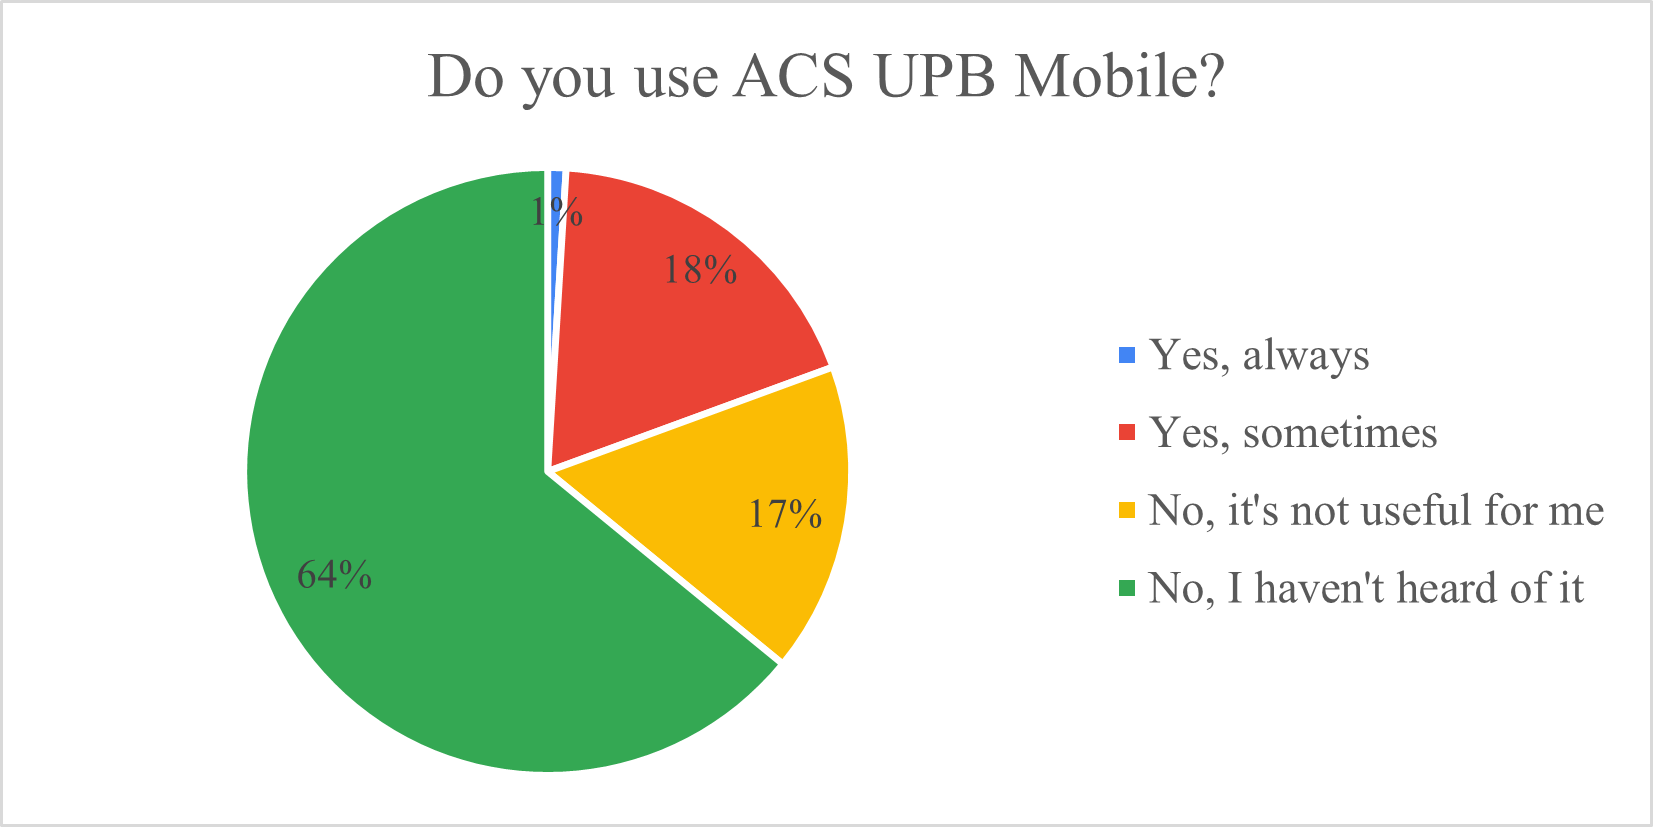
\includegraphics[width=\textwidth]{figures/charts/acs_upb_mobile.png}
            \caption{Use of ACS UPB Mobile}
            \label{4:fig:acs_upb_mobile}
        \end{figure}
        
        Given the fact that classes at \acrshort{upb} have been mostly online in the past two years due to the pandemic, we also wanted to understand for how long our survey responders have had in-campus, physical classes. We believed this may affect their view on the need for campus navigation. As seen in figure \ref{4:fig:semesters}, more than half of the students who responded have had only one semester of in-campus classes or even less. However, based on our data, we have not found a significant difference in responses from these students compared to the other groups. This indicates that issues with campus navigation are similar before and after the pandemic.
            
        \begin{figure}[!ht]
            \centering
            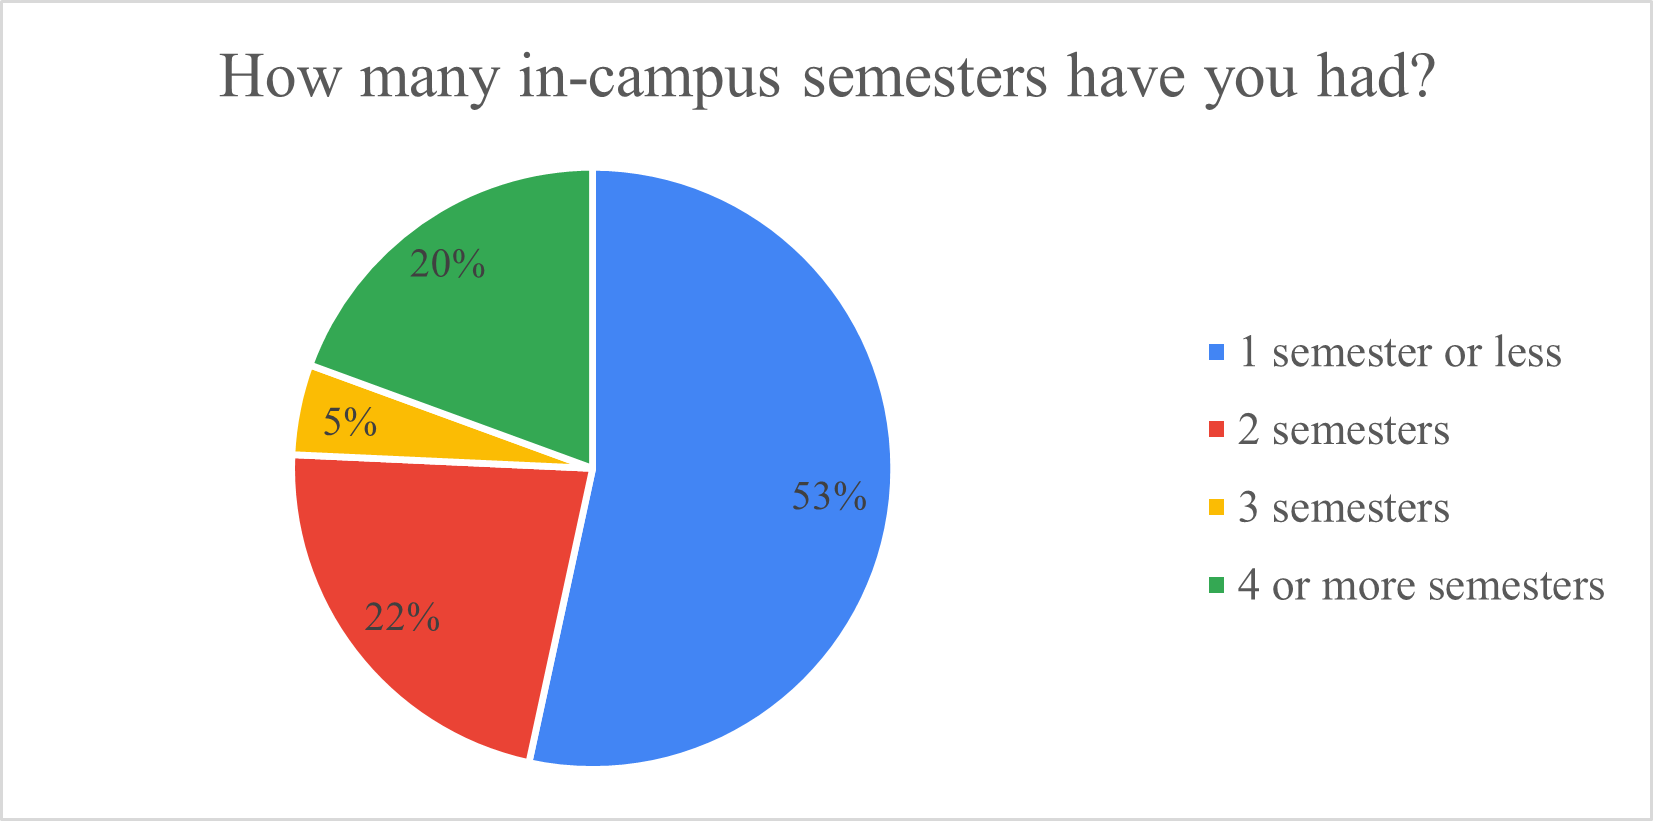
\includegraphics[width=\textwidth]{figures/charts/semesters.png}
            \caption{In-campus semesters for survey responders}
            \label{4:fig:semesters}
        \end{figure}
        
        We also used a Likert scale from \textit{Not important} to \textit{Very important} to assess what kind of information would be important to include in a campus map. The chart in figure \ref{4:fig:map_features} assigns a score from -1 to +2 to each level on the scale, and adds up the survey responses in order to display a reverse ranking of potential information that could be present on the map, based on the features we listed in section \ref{1:functionalities}. The features are in descending order based on the following formula:
        
        \[ \sum_{n=1}^{103} response_n \cdot score(response_n) \]
        
        where $response_n$ is the \textit{n}th survey response for this question (one of \textit{Very important, Important, Somewhat important, Not very important} and \textit{Not important}), and $score$ is:
        
        $$
        score(response) = \left\{
            \begin{array}{ll}
                -1\text{, if } response = \text{"Not important"} \\
                -0.5\text{, if } response = \text{"Not very important"} \\
                0.5\text{, if } response = \text{"Somewhat important"} \\
                1\text{, if } response = \text{"Important"} \\
                1.5\text{, if } response = \text{"Very important"} \\
            \end{array}
        \right.
        $$
            
        \begin{figure}[!ht]
            \centering
            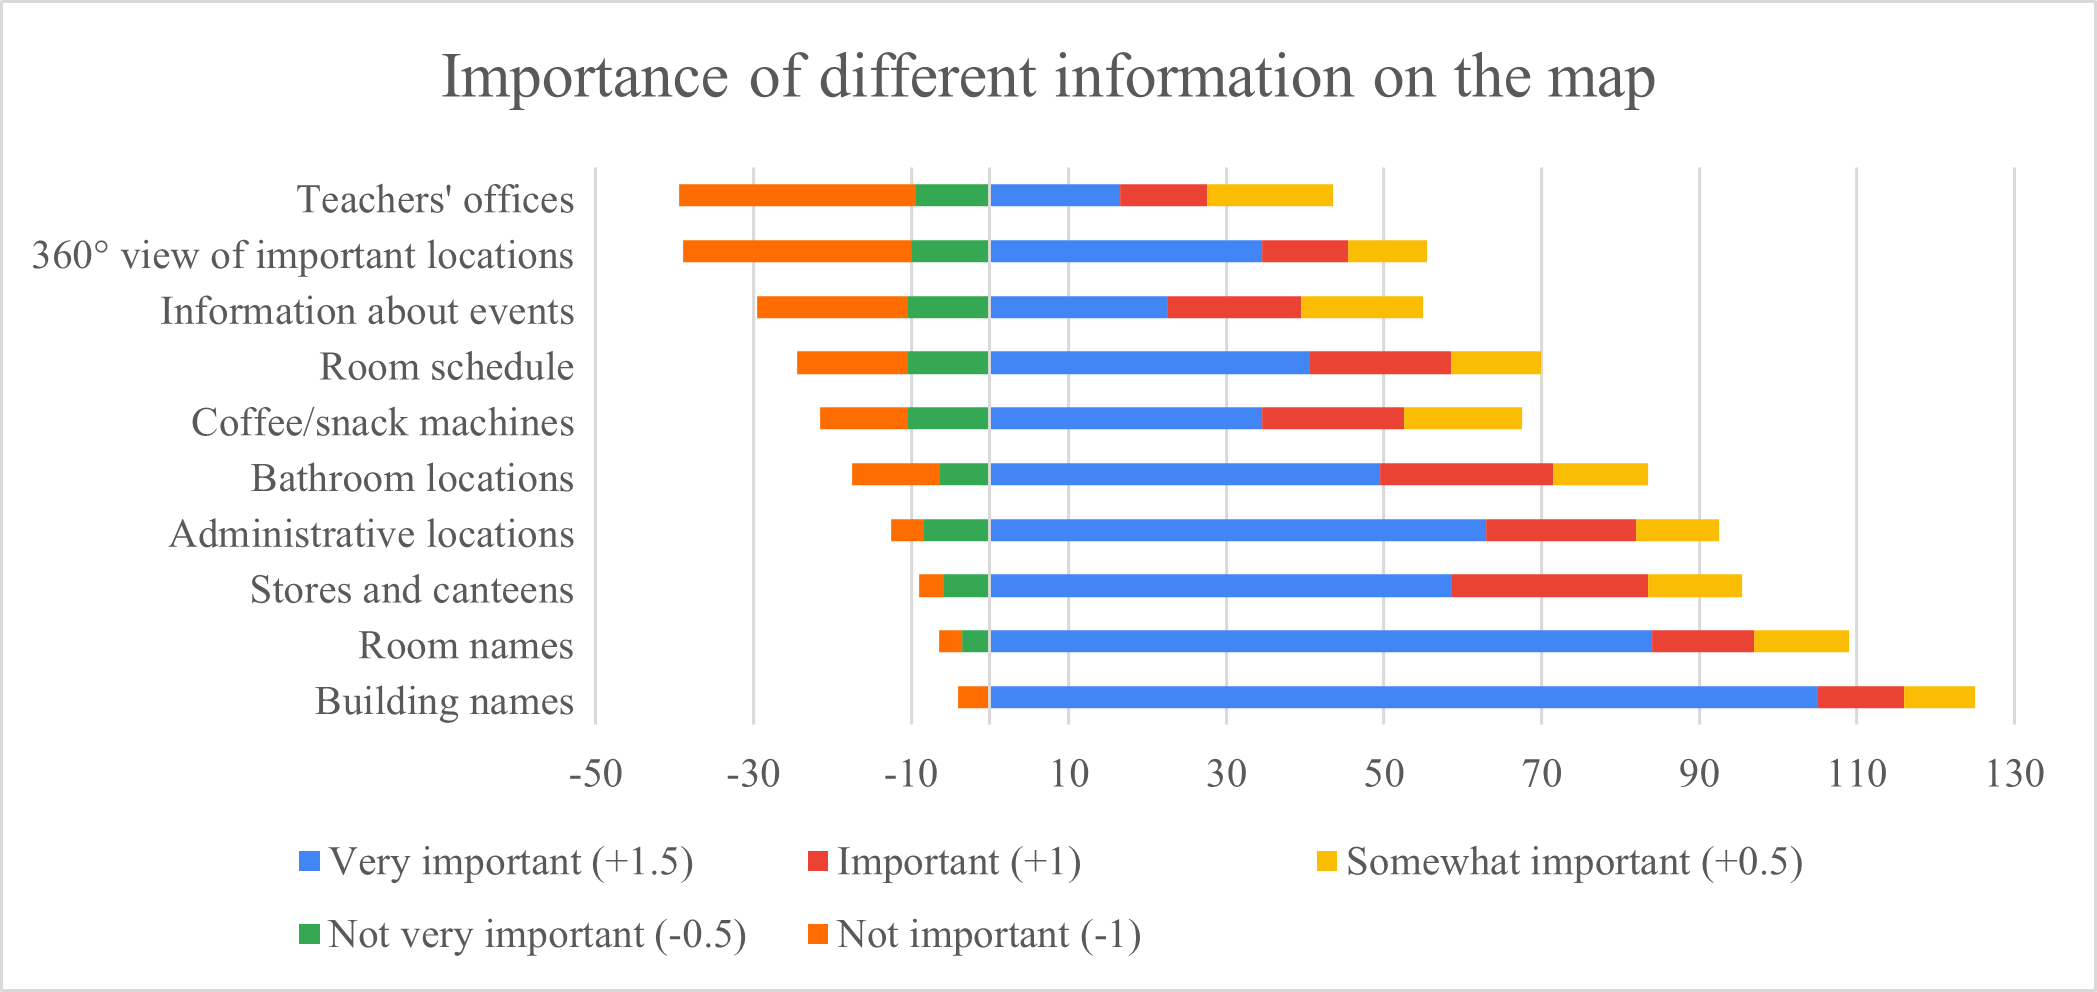
\includegraphics[width=\textwidth]{figures/charts/map_features.png}
            \caption{Importance of different information on the map}
            \label{4:fig:map_features}
        \end{figure}
        
        Based on this ranking system, by far the most important pieces of information that need to be on the map are the names of the campus buildings, corresponding to outdoor navigation. About 20 points away in the ranking are room names, corresponding to basic indoor navigation, as we have expected. In terms of \acrshort{poi}s on the map and another 20 points away, administrative locations such as the secretariat or the dean's office have a similar score to campus shops and canteens. Moving down another 20 points would be the locations of the bathrooms, which are lower than we expected - likely because they are usually reasonably easy to find anyway. Going down another 20-points-tick, we find another \acrshort{poi} - coffee \& snack machines. These have a similar importance score with information about the schedule of a specific room (e.g. what classes are taking place there at a specific time). Yet another 20 points further down the scale, we find information about other events taking place at specific locations. Ten points lower, and on the second to last importance position, we find the 360° views of important locations in the campus. Finally, another 10 points down the ranking and on the last position, we find information about the teacher's offices. It should be noted, however, that while the information on these last two positions are not important for students, they seem to carry more importance for aspiring high school students and university professors, respectively (see section \ref{4:interviews}).
        
        We also asked students what other information they would like to see on a map. Some of the suggestions for points of interest were \textit{elevators, student housing, parking spaces and print shops}.
        
        Several students also mentioned they would like to see access points and whether they are open or not (e.g. campus gates, building entrances, the location of the guard who keeps keys to the rooms).
        
    \subsection{Interviews} \label{4:interviews}
        We interviewed people from various user groups, including non-students:
        \begin{enumerate}
            \itemsep0em
            \vspace{-0.2cm}\item[(1)] a junior high school student aspiring to apply to UPB next year (and their mother, who joined the interview as well)
            \vspace{-0.2cm}\item[(2)] a professor at ACS
            \vspace{-0.2cm}\item[(3)] a computer science student from another university, who participated in events in our campus such as PoliJobs
            \vspace{-0.2cm}\item[(4)] a member of the ACS student league (LSAC)
        \end{enumerate}
        
        Both the high school student and their parent (1) were very interested in the 360° views of campus locations, as they wanted to see what learning there would be like. None of the other interviewees found this feature particularly useful, which matches the insight from the survey. They were also interested in understanding how to enter the campus and reach the location for the extracurricular maths classes taking place as prep for the entrance exams.
        
        The ACS professor said navigation would probably not be very useful for them as they already know most of the locations they would want to go to. However, they mentioned they sometimes forget which office some other professors are in (especially in the PRECIS building), and that having an accessible list with their office locations would be useful. They mentioned occasionally using the cs.pub.ro website to view this information. Once again, none of the other users interviewed found this information particularly useful.
	    
	    Interviewee (3) mentioned they had difficulty reaching the in-campus locations for the events they participated in, especially the library. This was mostly due to them not being familiar with the campus at all, considering they only came for a few visits. When asked if they would install an app especially to navigate in-campus at an event, they were hesitant. They eventually said they might have still resorted to asking around and using Google Maps over having to install another app.
	    
	    Interviewee (4) was excited about the possibilities that a campus navigation app could have, and mentioned a recent treasure hunt that the student league organised. They suggested that having a special app that would encourage people to participate and give them points when they reach certain locations would have been very useful. Furthermore, they also suggested that the app may be useful for high school students when they come to sign up for the admittance exam.
         
    \subsection{Demos} \label{4:demos}
        
        We invited a group of 5 students to test our proof of concept applications and provide feedback. We selected a diverse group:
        \begin{enumerate}
            \itemsep0em
            \vspace{-0.2cm}\item[(1)] a 1st year BSc student who hasn’t used either UPB Campus or ACS UPB Mobile
            \vspace{-0.2cm}\item[(2)] a 2nd year BSc student, a group leader who regularly uses ACS UPB Mobile and UPB Campus
            \vspace{-0.2cm}\item[(3)] a 4th year BSc student who doesn’t use either app
            \vspace{-0.2cm}\item[(4)] a 4th year BSc student who contributes to the ACS UPB Mobile development
            
            
            \vspace{-0.2cm}\item[(5)] a 2nd year MSc student who had most classes remote in the past two years, and doesn’t use either app
        \end{enumerate}
        
        \subsubsection{Impl. \#1: Flutter \& Google Maps SDK for Unity}
        
            First, we gave the testers a version of ACS UPB Mobile with the integrated campus map feature.
            The students who have not used ACS UPB Mobile before took time to explore other features in the app before getting to the map. Testers (1), (2) and (4) all noted that the map feature stands out as having a very different style and “feel” to the rest of the app. All testers noticed that the performance is pretty slow when opening up the map page. Tester (3) expressed that they believe “it’s easier to just use a photo of the map”. Tester (5) pointed out that ACS UPB Mobile looks like it may be useful, but the map feature itself wouldn’t really be useful for long. Finally, tester (2) said they consider UPB Campus to be easier to use and more intuitive.

        \subsubsection{Impl. \#2: Indoor (3D) navigation using NavMesh}
        
            Subsequently, we showed each tester a demo of the NavMesh-based 3D campus navigation. All testers expressed excitement upon seeing a 3D model of a building they are familiar with, and liked the comprehensive path it shows to the destination. They also asked to pan around the building so they can see it better. Testers (3), (4) and (5) mentioned they don’t find the third-person view to be very useful, and that being able to view the building from above and pan around it would be enough to understand the path.

        \subsubsection{Impl. \#3: Outdoor (3D) navigation with MapsModelsImporter}
        
            We then showed the testers the demo of the MapsModelsImporter approach. Except for (5), all testers preferred the view before (the simple building shape) to this more detailed map. Some mentioned the details are too distracting, and you can’t see the path very well. All testers mentioned that GPS localization should be part of every implementation, even if not entirely accurate. Tester (2) considered this to be similar to UPB Campus, but a bit more “overkill”.
        
        \subsubsection{Impl. \#4: AR-powered indoor navigation}
        
            Finally, we gave our testers the demo for AR-based indoor navigation. None of them had used this kind of navigation system before. When asked whether they knew Google Maps had this feature, tester (4) answered that they were aware of it, but hadn't tried it before; all other testers hadn't heard of this feature at all.
            Tester (1) found this feature very useful, and shared that they consider themselves bad at reading maps in general. They found this navigation approach more intuitive than following a map. The other testers said this approach "might" be useful, but that they would mostly opt for using a regular map or one of the other approaches instead. They felt uncomfortable having to walk around with a camera pointed at their surroundings.
